\documentclass[tikz,border=12pt]{standalone}
% Shared visual language for standalone EMT block diagrams.
\usepackage{amsmath}
\usetikzlibrary{arrows.meta,backgrounds,calc,fit,positioning}

\tikzset{
    emt diagram/.style = {>={Stealth[length=2.4mm]}},
    line/.style        = {semithick, rounded corners=6pt},
    block/.style       = {draw, semithick, fill=white,
                          minimum height=1cm, minimum width=2.3cm},
    hblock/.style      = {block, minimum width=2.24cm, minimum height=1.3cm},
    vblock/.style      = {block, minimum width=1.3cm, minimum height=2.24cm},
    sum/.style         = {draw, semithick, fill=white, circle,
                          inner sep=2.6pt},
    signal/.style      = {circle, fill, inner sep=1.4pt,
                          label distance=3pt},
    sig/.style         = {font=\small},
    pm/.style          = {font=\scriptsize},
    wire jump/.style   = {line,
                          preaction={draw=white, line width=3pt,
                                     line cap=round}},
    enclosure/.style   = {draw, dashed, semithick, rounded corners=4pt},
    operator enclosure/.style = {enclosure, inner xsep=7mm, inner ysep=6mm}
}


\begin{document}
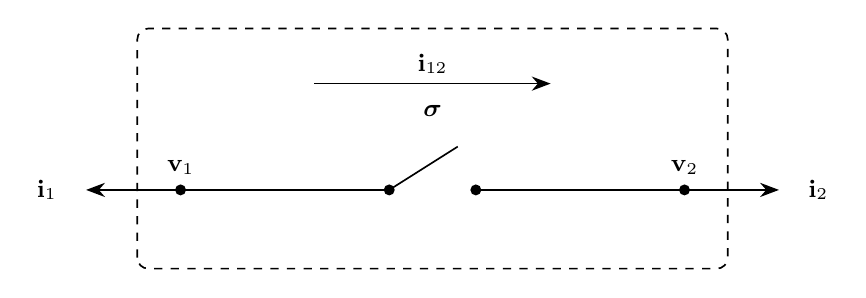
\begin{tikzpicture}[emt diagram]

% ================= Ideal switch contact =================
\coordinate (left contact) at (-0.55, 0);
\coordinate (right contact) at (0.55, 0);
\draw[line] (left contact) -- (0.32, 0.55);
\node[signal] at (left contact) {};
\node[signal] at (right contact) {};
\node[sig] at (0, 1.0) {$\boldsymbol{\sigma}$};

% ================= Terminal rails and bus injections =================
\draw[->, line] (left contact) -- (-4.4, 0);
\draw[->, line] (right contact) -- (4.4, 0);
\node[sig, anchor=east] at (-4.65, 0) {$\mathbf{i}_1$};
\node[sig, anchor=west] at (4.65, 0) {$\mathbf{i}_2$};

% ================= Terminal voltages =================
\node[signal, label={[sig]above:$\mathbf{v}_1$}] at (-3.2, 0) {};
\node[signal, label={[sig]above:$\mathbf{v}_2$}] at (3.2, 0) {};

% ================= Branch-current direction =================
\draw[->, line] (-1.5, 1.35) -- (1.5, 1.35);
\node[sig, anchor=south] at (0, 1.35) {$\mathbf{i}_{12}$};

% ================= Model enclosure =================
\draw[enclosure] (-3.75, -1.0) rectangle (3.75, 2.05);

\end{tikzpicture}
\end{document}
